\chapter{Stockage des boîtes et visualisation}
Trois problèmes majeurs apparaissent dans la réalisation du logiciel de visualisation. La première est bien entendu la gestion d'une très grande quantité de boîtes lors de l'affichage. Il est en effet nécessaire d'offrir un accès rapide aux informations des boîtes dans la fenêtre. La seconde est la gestion des filtres sur ces mêmes boîtes. Et le troisième apparait lors du changement des variables étudiées (changement des dimensions visualisées).

\section{\'Etude d'une solution possible : le QuadTree}
\paragraph{}Une des solutions qui permettrait d'offrir une visualisation fluide du pavage tout en répondant aisément au document de spécifications serait de représenter le pavages sous une forme de quadtree pour deux dimensions ou octree pour trois dimensions.

\paragraph{Le QuadTree}\label{par:QT}consiste à découper récursivement un espace fini en deux dimensions en quatre parties égales. Chacune de ces parties sont stockées dans un nœud. On itère ce mécanisme sur chacun de ces nœuds jusqu'à isoler spatialement les éléments recherchés.
\begin{figure}[htbp]
\centering
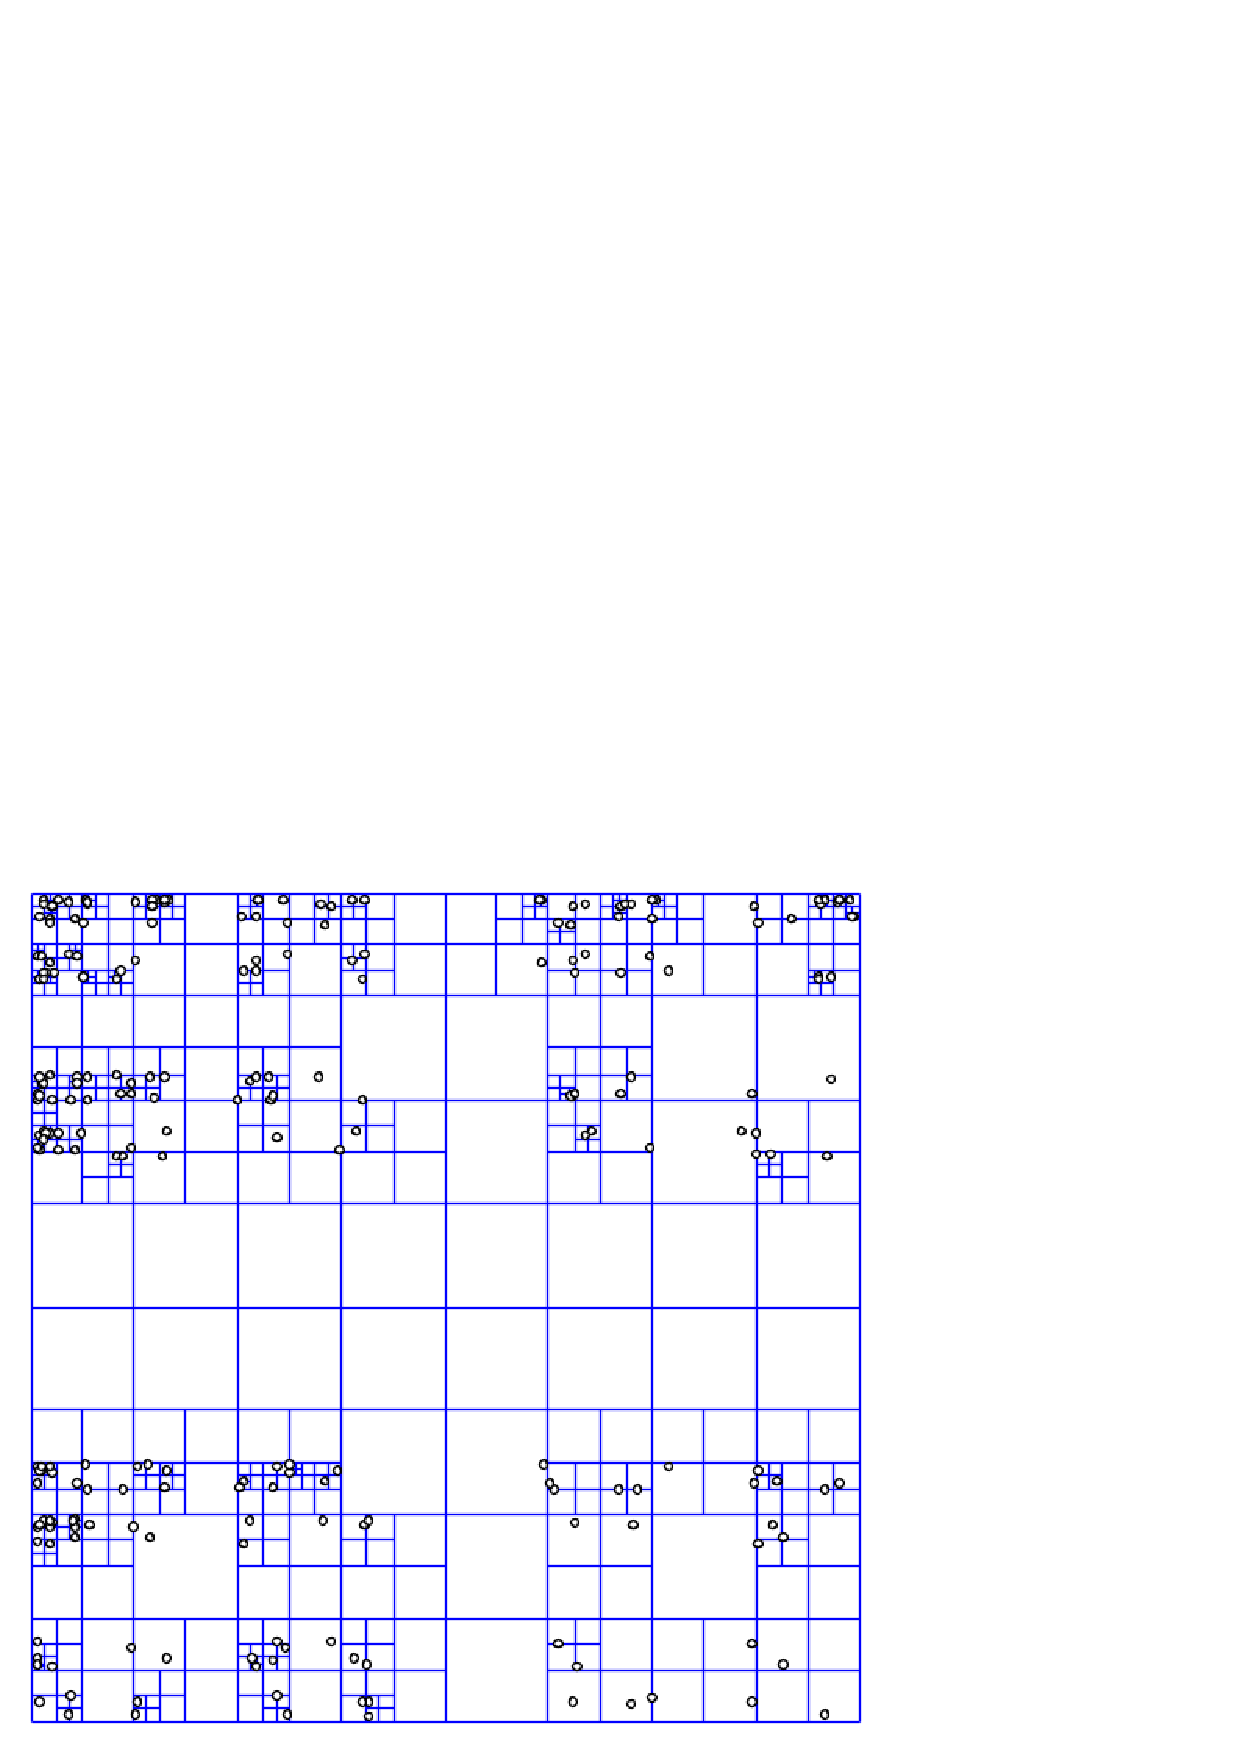
\includegraphics[scale=0.50]{quadtree}
\caption{Représentation d'un quadtree}
\end{figure}
Cette strucure pourrait être utilisée pour déterminer la position des boîtes dans l'espace selon la méthode suivante :
\begin{itemize}
\item []Si un des nœuds du quadtree ne contient aucune boîte ou qu'il est entièrement inclus dans un ensemble de boîtes alors il n'est plus nécessaire de le subdiviser. Ce nœud contiendra donc une référence sur chacune de ces boîtes.
\begin{figure}[htbp]
\centering
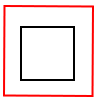
\includegraphics[scale=0.20]{img/QT1}
\end{figure}
\item \`A contrario si un nœud du QuadTree contient une des bornes d'une des boîtes, alors il est nécessaire de subdiviser ce nœud.
\item On arrête aussi de diviser les nœuds lorsque l'on arrive à une précision inférieur à la précision d'affichage (taille d'un pixel).
\end{itemize}

L'octree repose sur le même principe mais étendu à trois dimensions. L'espace est donc découpé en huit parties à chaque fois.

Cette structure est particulièrement intéressante pour la visualisation du pavage. En effet pour une fenêtre de visualisation donnée, il est très simple et rapide d'extraire la sous-arborescence correspondante à l'espace visualisé et permet aussi de ne pas afficher les objets trop petits.

Le problème de cette méthode est essentiellement du à la construction. La structure devra découper en la plus petite feuille possible au niveau des bornes des boîtes ce qui va nécessairement entrainer la construction d'un grand nombre de feuilles. Ce problème est particulièrement gênant puisque si l'on cherche à localiser une boîte de dimensions 1 sur 1 avec la précision donnée par défaut par Realpaver de $10^{-16}$, on se retrouve avec au moins $4 \times 10^{16}$ feuilles. On peut optimiser l'algorithme de construction en considérant que si un des nœuds contient l'intégralité ou une partie d'une seule boîte, il n'est plus nécessaire de subdiviser. La recherche d'une seule boîte étant immédiate.

Un autre problème apparait lorsque l'utilisateur souhaite changer les variables visualisées dans l'outil. Si l'on reste sur une structure du type QuadTree ou octree, il sera nécessaire de recalculer entièrement l'arbre.

On pourrait alors supposer une structure similaire $k$-dimensionnelle\footnote{$k$ étant la dimension du problème fourni à Realpaver.} où chaque nœud possède $2^k$ nœuds. L'avantage d'une telle structure est que lorsque l'on désire changer les variables de visualisation, le calcul est déjà effectué.

\paragraph{} Malgré le fait que le QuadTree pouvait être une structure intéressante, le nombre de feuilles créées est bien trop important et ne peut donc pas être utilisé.

\section{\'Etude d'une seconde solution : le R-tree}
\paragraph{Le R-tree} est une structure de données utilisée pour stocker des informations $k$-dimensionnelles. Le principe est le suivant :
\begin{itemize}
 \item Un noeud de l'arbre correspond à une boîte non-solution du pavage.
 \item Chaque boîte peut contenir entre $m$ et $M$ sous-boîtes entièrement incluses. Avec $m\leq \frac{M}{2}$.
 \item Une feuille de l'arbre est une boîte ne contenant que des boîtes solution du pavage.
 \item L'arbre est équilibré.
\end{itemize}

La figure \ref{fig:rtree} donne une bonne idée du principe des R-trees\cite{wiki}:
\begin{figure}[htbp]
\centering
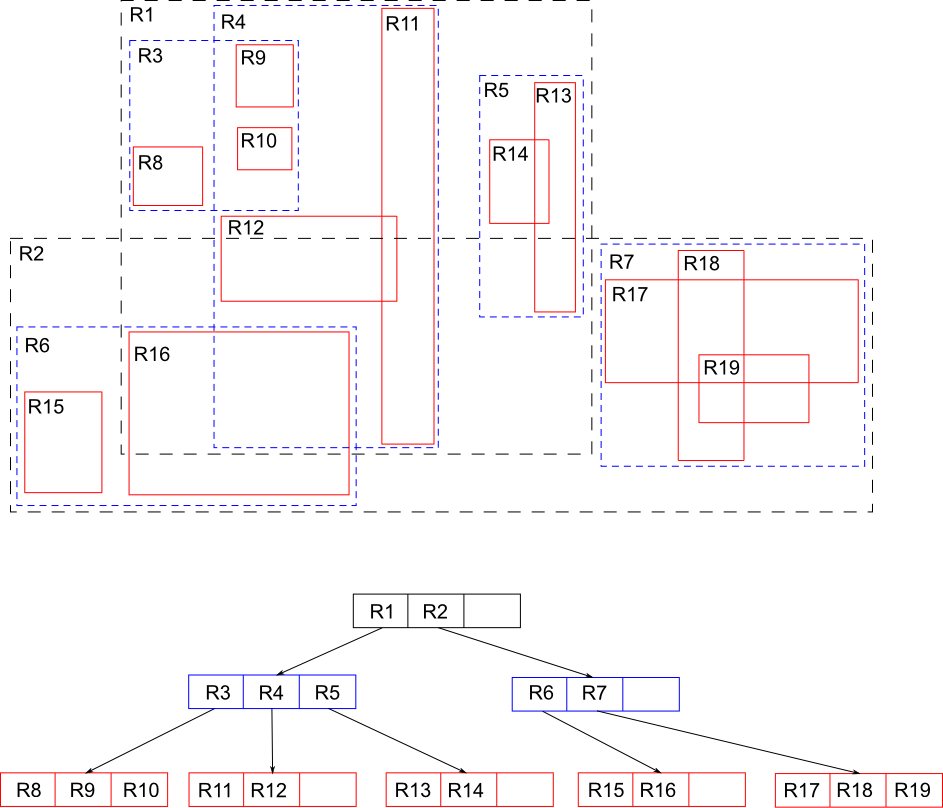
\includegraphics[scale=0.50]{rtree}
\caption{Représentation d'un R-tree}
\label{fig:rtree}
\end{figure}

Pour plus de détails sur le R-tree on pourra se référer à l'article de A. Guttman \cite{Guttman}

\paragraph{} Une telle structure semble bien plus intéréssante en terme d'occupation mémoire. En effet le nombre de feuilles de l'arbre est au pire égale à $\frac{N}{m}$. Cependant on peut se demander si rechercher une fenêtre de visualisation serait efficace. En effet il est nécessaire de parcourir toutes les boîtes dont l'intersection est non nulle avec la fenêtre. De nombreuses analyses ont été effectuées sur le sujet. On pourra se reporter à une analyse de performances sur les Priority R-trees \cite{PRTree}.

